\chapter{Mathematical Background}
\label{MathBack}

In order to understand the mathematical concepts behind the encryption algorithms described here, some basic concepts are explained here. However, you should have a basic knowledge of linear algebra and polynomial calculus.

\section{Lattice}

% Based on \cite{LatticeTutorial}.

All of the algorithms discussed in this thesis are based on lattices, which is why we will briefly focus on them in more detail. In general, lattices behave like any other vector space, but they only consist of discrete vectors. This means that the vectors only contain integers and not real numbers as in a vector space.

Let $B = \{b_1, b_2, \ldots, b_m\}$ be a set of linearly independent vectors of $\mathbb{R}^n$. The lattice $L$ generated by $B$ is the set of integer linear combinations of $B$. $B$ is called the basis of the lattice $L$. That is,
$$L(B) = \{a_1b_1 + \ldots + a_mb_m | a_1, \ldots, a_m \in \mathbb{Z}  \} \subset \mathbb{R}^n$$


Using a matrix $B$, which contains the basis vectors as column vectors, we can generate $L$ equivalently.

$$L(B) = \{Bx | x \in \mathbb{Z}^m  \} \subset \mathbb{R}^n$$

As in this definition, the integer $n$ is the \textbf{dimension} of the lattice and $m$ is its \textbf{rank}. If $m = n$, then $L$ is a \textbf{full-rank} lattice, which is the usual case in this thesis. 

An example of a lattice based on a basis $B$ and all the points that can be created with it, also called the \textbf{span}, can be seen in the figure \ref{fig:latticeGrid}.

\begin{figure}[h]
  \centering
  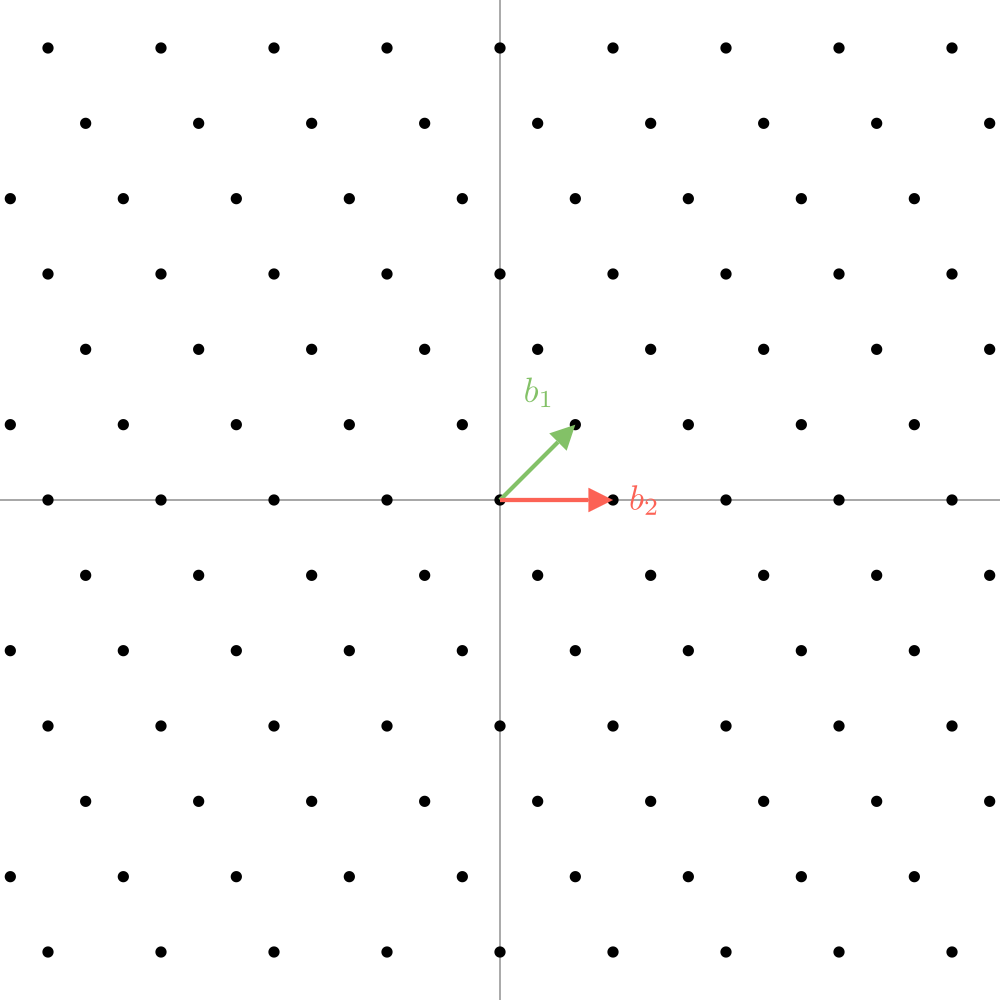
\includegraphics[scale=0.2]{images/LatticeGrid.png}
  \caption[Span of an Lattice]{The span of an two-dimensional lattice with basis  $B = \{b_1, b_2\}$.}
  \label{fig:latticeGrid}
\end{figure}

% Nur dann benötigt wenn ich genauer auf die Funktionsweise von LWE eingehen will
% \section{Shortest Vector \& Closest Vector Problem}


\section{Integer \& Polynomial Rings with modulus}
This section is based on \cite{Algebra}.

\subsection*{Rings}
A ring is a set $R$ on which addition ($+$) and multiplication ($\cdot$) can be performed and results in a new Element, which is also part of the set R.
\begin{center}
  $ +: R+R\rightarrow R$ (Addition) and $\cdot: R \cdot R \rightarrow R$ (Multiplication)
\end{center}

These calculations need to fulfill the following conditions:
\begin{description}
  \item for addition: $R$ is an abelian group
        \begin{itemize}
          \item Associative property: $(a+b)+b = a+(b+c) | a,b,c \in R$
          \item Commutative property: $a+b = b+a | a,b \in R$
          \item Additive identity: There exists and element $0 \in R$ so that $a+0 = a | a \in R$
          \item Additive inverse: For each $a \in R$ there is an $-a \in R$ so that $a+(-a)=0$
        \end{itemize}
  \item for multiplication: R is an monoid
        \begin{itemize}
          \item Associative property: $(a\cdot b) \cdot b = a \cdot(b\cdot c) | a,b,c \in R$
          \item Multiplicative identity: There exists and element $1 \in R$ so that $a \cdot 1 = 1 \cdot a = a | a \in R$
        \end{itemize}
  \item Addition and Multiplication are distributive
        \begin{itemize}
          \item  $a\cdot (b + c) = a\cdot b + a\cdot c | a,b,c \in R$
          \item  $(a + b) \cdot c= a\cdot c + b\cdot c | a,b,c \in R$
        \end{itemize}
\end{description}

A ring is also called commutative if the multiplication is also commutative. For example, the ring over all integers $\mathbb{Z}$ is a commutative ring.

\subsection*{Modular arithmetic on Rings}

Congruence arithmetic, or modular arithmetic, is the term used to describe arithmetic with remainders when dividing integers. In everyday life, this is mainly encountered in connection with clocks. After 60 minutes, the minute hand returns to the same position as before. 

More generally, this can be described as $a \equiv b \mod n | a,b \in \mathbb{Z}, n \in \mathbb{N}$, where $n$ is the module by which $a$ and $b$ are divided until the remainder of both is less than $n$. If $a$ and $b$ are then equal, they are congruent. Or in a more mathematical expression: If there is a $k$, such as $a-b = k\cdot m$, then $a$ and $b$ are congruent.

An congruence relation with module $n$ on the set $\mathbb{Z}$, has the following properties:
% Based on \cite{Algebra} Seite 13.
$k,n \in \mathbb{N}$ and $a, a', b, b', c \in \mathbb{Z}$
\begin{enumerate}
  \item $a \equiv a \mod n$ (Reflexivity)
  \item $a \equiv b \mod n$ if $b \equiv a \mod n$ (Symmetry)
  \item If $a \equiv b \mod n$ and $b \equiv c \mod n$ then $a \equiv c \mod n$ (Transitivity)
  \item If $a \equiv a' \mod n$ and $b \equiv b' \mod n$ then $a+b \equiv a'+b' \mod n$
  \item If $a \equiv a' \mod n$ and $b \equiv b' \mod n$ then $a\cdot b \equiv a'\cdot b' \mod n$
  \item If $c$ and $n$ are coprime and $c \cdot a \equiv c \cdot b \mod n$ then $a \equiv b \mod n$
  \item If $a \equiv b \mod k\cdot n$ then $a \equiv b \mod n$
\end{enumerate}

The congruence class is the set of all numbers for an integer $a \in \mathbb{Z}$ modulus $n$ that produce the same remainder. It is defined as
$$[a]_n = \{b \in \mathbb{Z} | a \equiv b \mod n\}$$.

It follows that two numbers are congruent if both congruence classes are equal:

$$a \equiv b \mod n \Leftrightarrow [a]_n = [b]_n$$

With this we can create a set of all congruence classes modulo $n$:
$$\mathbb{Z}_n = \mathbb{Z}/n = \mathbb{Z} \mod n = \{[a]_n | a = 0, 1, \dot, n-1 \}$$.

For example, $Z_3 = \{[0]_3, [1]_3, [2]_3\}$. With addition and multiplication it is possible to create a commutative ring from $\mathbb{Z}_n$.
\begin{center}
    $[a]_n + [b]_n = [a+b]_n$ (addition) and $[a]_n \cdot [b]_n = [a\cdot b]_n$ (multiplication)
\end{center}

This allows to create finite rings $\mathbb{Z}_n$ for every natural number $n$ with $n$ elements in each ring and to perform calculations inside these ring. For example, an ring with $n=60$ can be created, which represents the minutes in every hour. If the minute hand shows now $48$ and we want to know where it is after $3$ times $13$ minutes, we can calculate it like:
$$[48]_{60} + [3]_{60}\cdot [13]_{60} = [48+3\cdot 13]_{60} = [87]_{60} = [27]_{60}$$